\section{Accessibilità}

\subsection{Cecità}
Per testare il sito rispetto agli screen reader è stata utilizzata l'estensione Fangs del browser Firefox.\\
L'utilizzo di Fangs ha permesso di constatare che:
\begin{itemize}
	\item tutti i link sono catturati;
	\item cambi lingua e tabelle sono gestiti correttamente;
	\item la corretta visualizzazione degli header delle varie pagine;
	\item ogni immagine ha il rispettivo testo alternativo.
\end{itemize} 

\begin{figure}[H]
  \centering 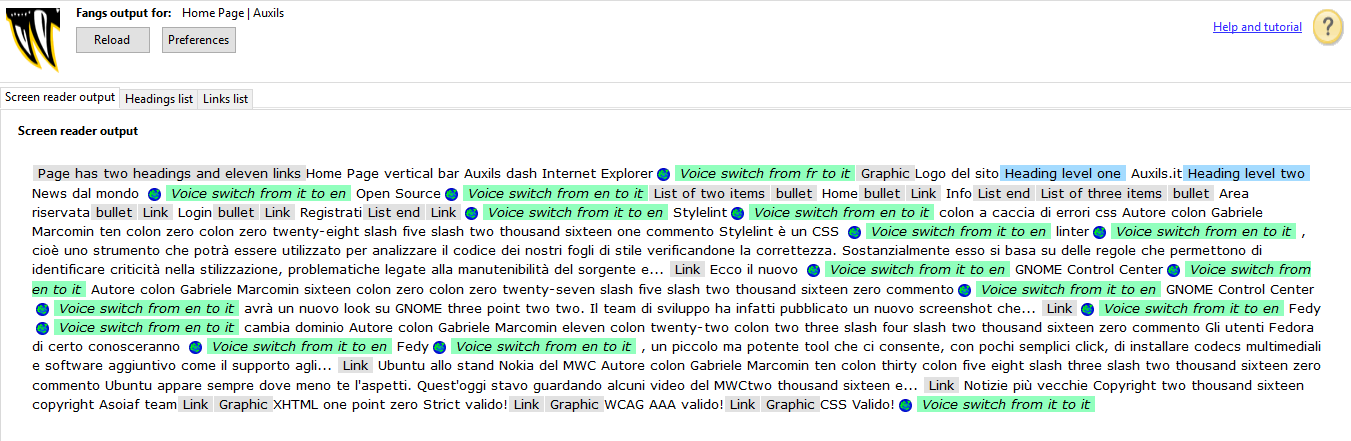
\includegraphics[width=0.8\textwidth]{images/fangs.png}
  \caption{Home visualizzata con Fangs}
\end{figure}

\begin{figure}[H]
  \centering 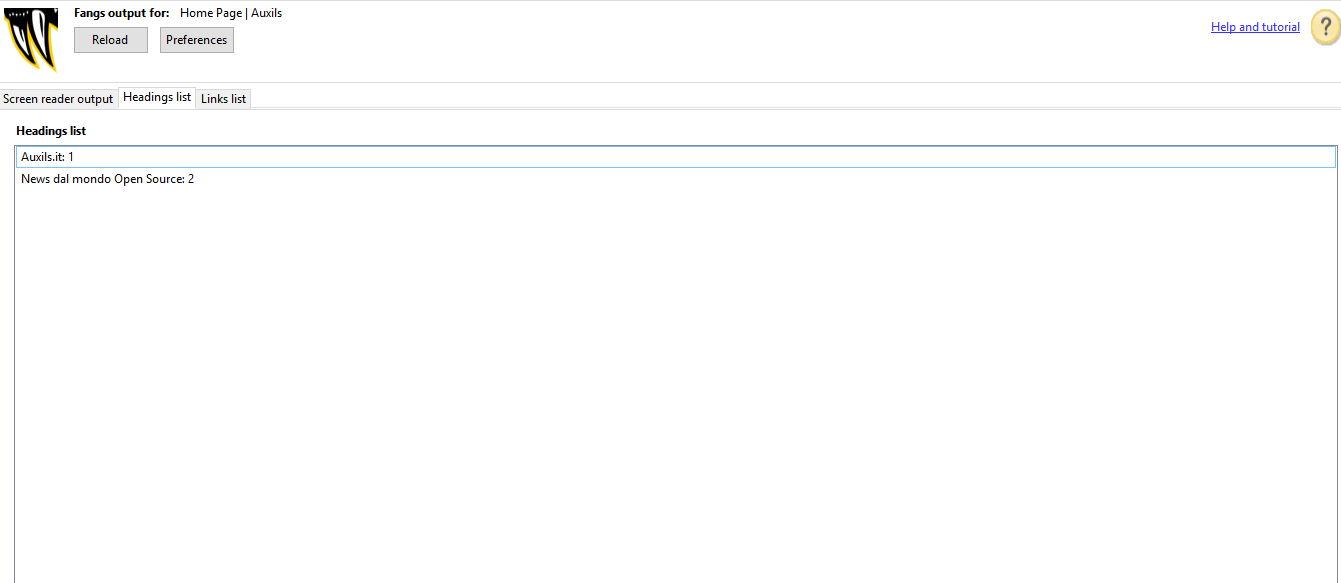
\includegraphics[width=0.8\textwidth]{images/fangsHeader.png}
  \caption{Lista degli header della home visualizzati da Fangs}
\end{figure}
	
\begin{figure}[H]
  \centering 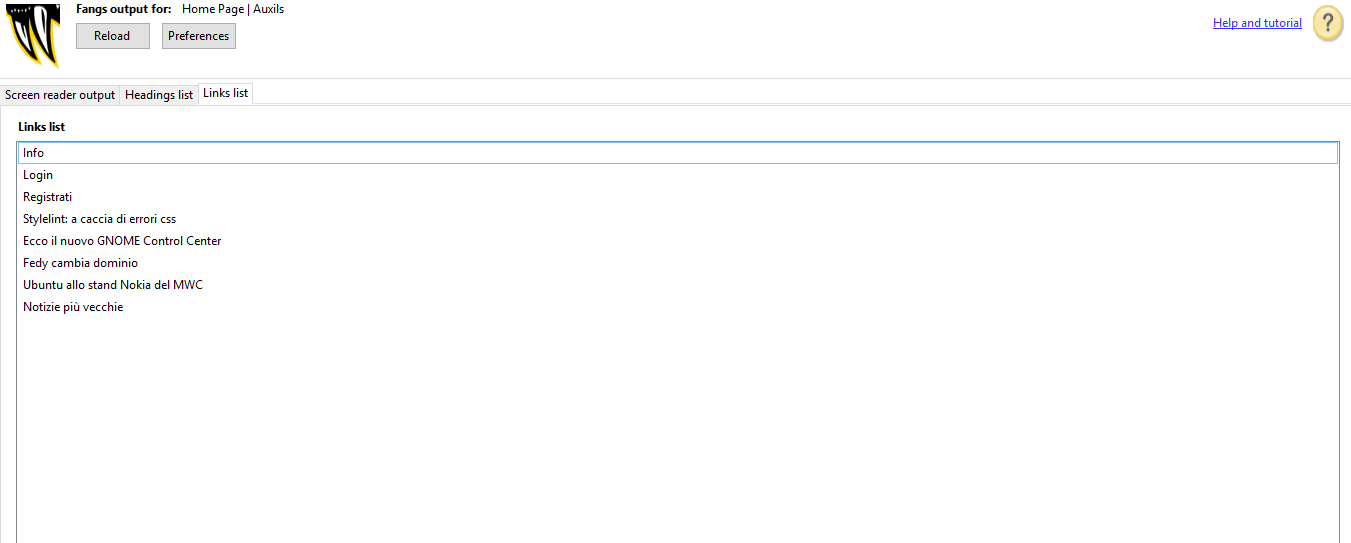
\includegraphics[width=0.8\textwidth]{images/fangsLink.png}
  \caption{Elenco di link contenuti nella home visualizzati da Fangs}
\end{figure}

\subsection{Cecità ai colori}
Al fine di testare che il sito sia accessibile anche da persone che hanno problemi nella corretta visualizzazione dei colori, si è utilizzato ImageJ e l'estensione Vischeck.
Tale estensione permette di visualizzare come viene percepita un'immagine da chi soffre di cecità ai colori. Ogni pagina è stata testata in modo da verificare che sia visualizzabile correttamente con il medesimo grado di contrasto da tutte le tipologie di utenti.

\begin{figure}[H]
		\centering 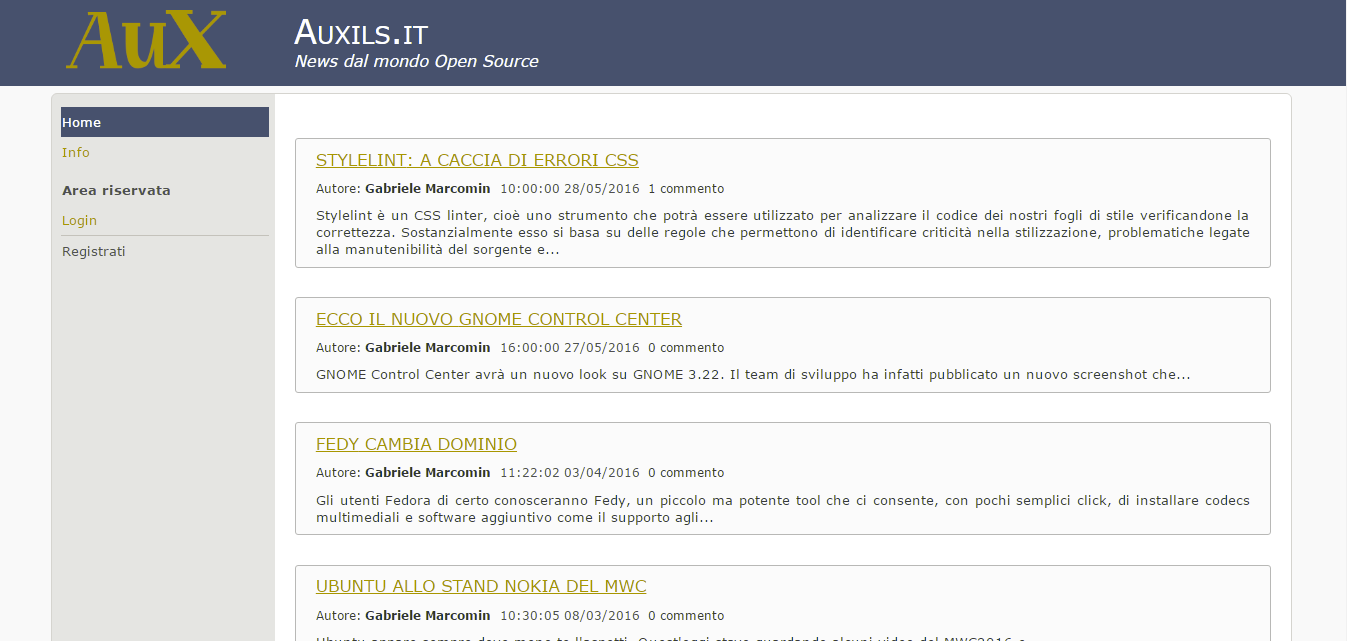
\includegraphics[width=0.9\textwidth]{images/deute.png}
		\caption{Home vista da chi soffre di deuteranopia}
\end{figure}
	
\begin{figure}[H]
		\centering 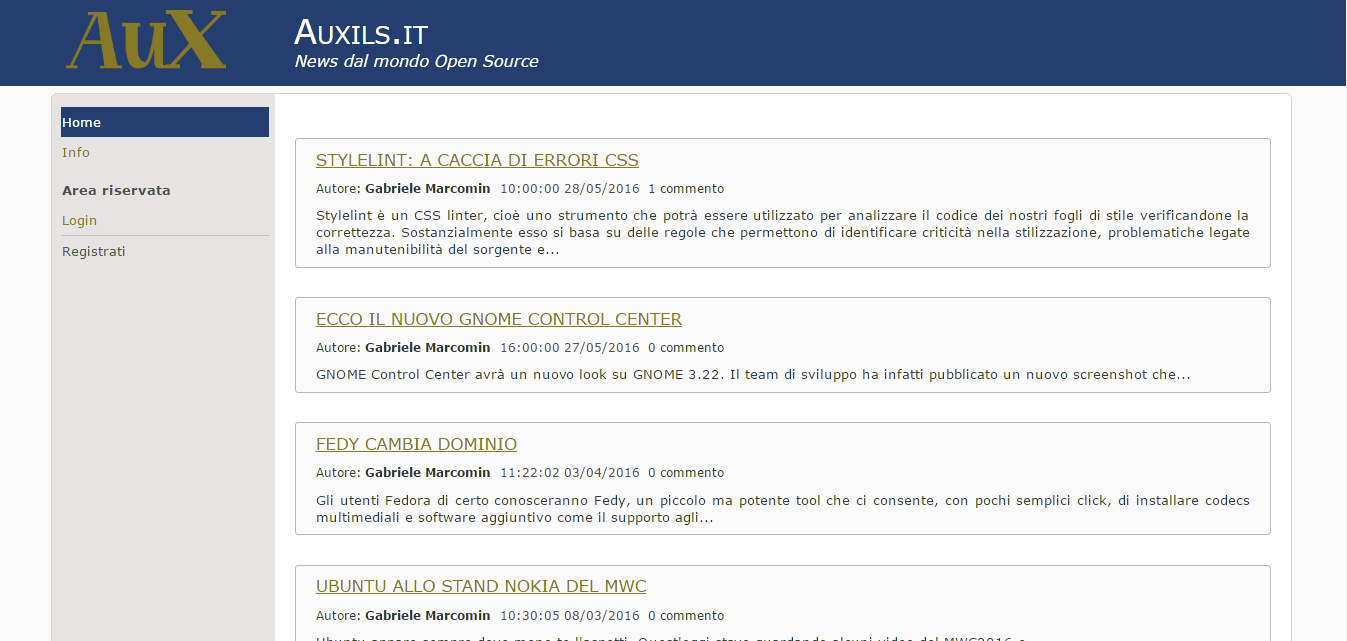
\includegraphics[width=0.9\textwidth]{images/proto.png}
		\caption{Home di pagina vista da chi soffre di protanopia}
\end{figure}
	
\begin{figure}[H]
		\centering 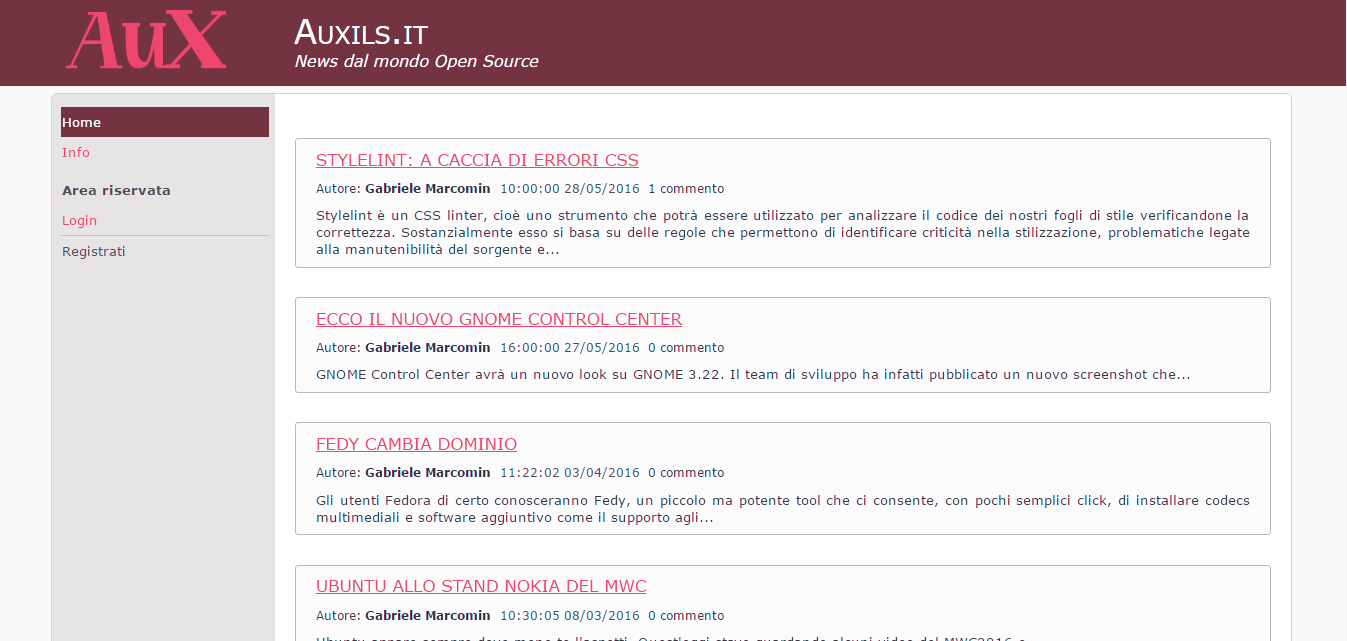
\includegraphics[width=0.9\textwidth]{images/trita.png}
		\caption{Home di pagina vista da chi soffre di tritanopia}
\end{figure}

\subsection{Form}
Durante la realizzazione dei vari form, sono stati tenuti i seguenti accorgimenti al fine di ottenere un buon grado di accessibilità ed usabilità generale:
\begin{itemize}
 \item ad ogni elemento input, di tipo text e textarea, è associata la relativa label con attributo for;
 \item ogni label di ogni campo obbligatorio ha come ultimo carattere il carattere *, per far notare meglio l'obbligatorietà del l'inserimento del campo;
 \item in caso di valori inseriti non validi, gli script Javascript e gli script cgi avvertiranno l'utente con dei messaggi. Come detto in precedenza, in caso di disattivazione di Javascript gli script perl visualizzeranno il medesimo messaggio per lo stesso tipo di errore occorso;
 \item l'utilizzo di fieldset e legend al fine di raggruppare e descrivere un insieme di campi.
\end{itemize}

\subsection{Linee guida per il testo}

Le regole per testi alternativi alle immagini sono le seguenti:
\begin{itemize}
 \item il testo deve presentare il contenuto e la funzione dell'immagine;
 \item alt ed eventuali descrizioni sotto l'immagine non devono presentare lo stesso contenuto;
 \item il testo degli alt e delle eventuali descrizioni deve essere breve e conciso;
 \item alt ed eventuali descrizioni non devono iniziare con "immagine di.." o simili.
\end{itemize}

Per tabelle le regole usate sono le seguenti:
\begin{itemize}
 \item l'utilizzo di caption per dotare la tabella di un titolo;
 \item l'utilizzo di summary per dotare una descrizione del contenuto alla tabella, al fine di aiutare gli utenti non vedenti a comprendere velocemente il contenuto della tabella senza doverlo vedere tutto per capirlo;
 \item l'utilizzo di th per fornire contesto alle varie celle della tabella.
\end{itemize}

\subsection{Tastiera}
Condizione necessaria, ma non sufficiente, ad un sito per essere accessibile è che possa essere navigato utilizzando solamente la tastiera. Ogni pagina è stata testata al fine di verificare che la condizione di navigabilità via tastiera sia sempre rispettata.\\
Non sono stati utilizzati tabindex per i link della barra di navigazione in quanto il sito possiede un flusso semplice e lineare.

\subsection{Total Validator}
Total Validator è una applicazione che permette di verificare l'accessibilità di una pagina web secondo alcuni parametri.\\
Le impostazioni scelte per Total Validator sono state le più stringenti, richiedendo un'accessibilità aderente allo standard WCAG 2.0 AAA.\\
L'esito delle verifiche è stato positivo allo standard, in quanto non sono stati rilevati errors o warnings.